\chapter{INTRODUÇÃO}

Pode-se definir mídias sociais como aplicações da Internet que permitem que
indivíduos mantenham um conjunto de conexões com outros usuários, e compartilhem
informações pessoais e conteúdos gerados através de redes digitais \cite{boyd2007}.
Tais redes sociais são baseadas no fluxo de informações que nem sempre são públicas,
e geralmente acontece através de infraestruturas privadas de entidades interessadas
em prover o serviço, como por exemplo o Facebook e o Google.

Em segurança computacional, pode-se definir privacidade como a capacidade de um
indivíduo controlar quais e como as informações relacionadas a ele podem ser
consumidas ou armazenadas, e para quais indivíduos estes dados podem ser divulgados.
\cite{stallings2010}. Além de garantir o direito à privacidade de seus usuários,
as redes sociais devem garantir a confidencialidade das informações que hospeda,
assegurando que dados privados são sejam expostos a indivíduos não autorizados.

Argumenta-se que o poder de um único grande provedor sobre um fluxo de dados
privados coloca em risco a privacidade de seus usuários, já que não garante a
confidencialidade das informações privadas. As críticas a estes provedores
geralmente são acentuadas pela falta de transparência na utilização dessas
informações que geralmente assume um papel comercial, como na identificação de
padrões de comportamento em suporte à publicidade.

\begin{figure}[!htbp]
	\centering
		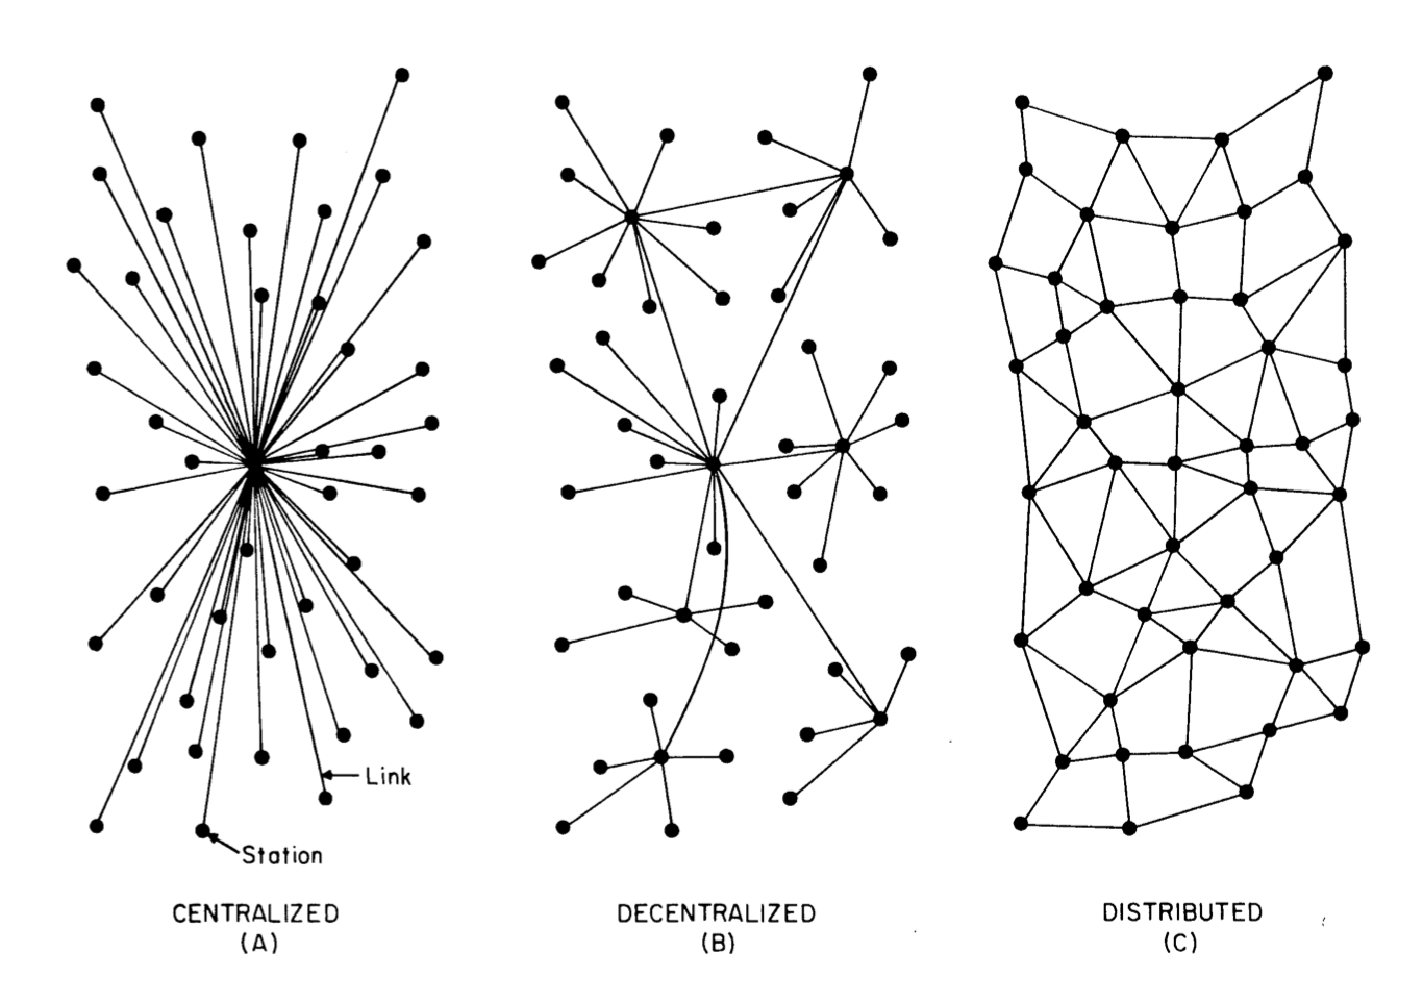
\includegraphics[keepaspectratio=true,scale=0.5]{figuras/org_redes.eps}
	\caption{Modelos conceituais de redes de comunicação \cite{baran1964}}
	\label{fig:org_redes}
\end{figure}

Uma alternativa à centralização do fluxo de dados privados é baseada no conceito
de redes descentralizadas, um dos padrões de organização de redes de comunicação.
Indica-se que em relação à organização de seus nós, redes de comunicação podem
assumir uma organização centralizada ou distribuída \cite{baran1964}. Como pode ser
visto na Figura \ref{fig:org_redes}, em contraste a redes centralizadas, uma rede
distribuída não depende de um único servidor central.

Redes sociais privadas, mesmo que providas por meio de infraestruturas
descentralizadas por questões de eficiência ou desempenho, conceitualmente respeitam
o modelo de uma rede centralizada. O nó central representa o provedor do serviço
enquanto os demais representam dos milhões de clientes. Adotar o modelo
descentralizado significa dividir os clientes entre provedores intermediários
conectados que ofereçam o mesmo serviço, garantindo a interoperabilidade.

Alguns autores também definem esta organização como uma rede federada, que é similar
à definição de redes descentralizadas de \cite{baran1964}, mas também é definida na
literatura como um conjunto de implementações interoperáveis que respeitam o modelo
cliente-servidor \cite{barocas2012}. Esta definição é importante por que generaliza
o conceito de federação para outros tipos de sistemas de comunicação que não redes
literais de computadores, e indica a propriedade de independência de extensão ---
qualquer entidade que garanta a interoperabilidade pode ser parte da federação.

A distribuição dos serviços contrapõe a existência de um único provedor, comum em
redes sociais fechadas como o Facebook e Twitter. A descentralização garante que o
armazenamento das informações não está restrito a apenas um proprietário. Mais
importante, a independência de extensão permite que qualquer indivíduo inclua um
novo servidor na federação, desde que respeite os critérios de interoperabilidade,
hospedando seus próprios dados. A descentralização do fluxo de dados privados
distribui a responsabilidade pela manutenção de confidencialidade, o que passa a não
depender de uma única entidade com intenções inexplícitas.

Por outro lado, a federação é fundada na capacidade de interoperabilidade entre
sistemas. Visto que o cenário provável envolve a comunicação entre sistemas
distintos em vários aspectos, é essencial considerar protocolos e padrões.

O objetivo deste trabalho é estudar a federação no contexto de redes sociais,
investigando quais os aspectos envolvidos na interoperabilidade destas mídias, e o
estado do esforço de padronização da interoperabilidade. Um segundo objetivo é
aprofundar esta análise no caso específico do Noosfero, uma rede social livre,
projetando e implementando uma prova de conceito de federação.

A utilização e padronização de protocolos de comunicação na interoperabilidade de
sistemas é introduzida no Capítulo \ref{chapter:2}, que aborda a utilização de
especificações na federação de sistemas, apresentando as iniciativas de padronização
nesse contexto. O Capítulo \ref{chapter:3} descreve o Noosfero e retrata o estado da
federação até a publicação deste trabalho, propondo a evolução da federação com
outras redes através de implementação com base no protocolo Diaspora. Por fim, o
Capítulo \ref{chapter:4} apresenta os resultados de parte dessa implementação,
enquanto o Capítulo \ref{chapter:5} conclui o trabalho apontando os próximos passos
para o desenvolvimento do projeto.
